\subsection{\label{subsec:FZV6}Zentriertes Gitter}
\textbf{\textit{a) Was versteht man unter einem zentrierten Gitter? 
Diskutieren Sie kurz die verschiedenen Möglichkeiten der Gitterzentrierung 
und geben Sie auch an, wie viele Gitterpunkte dann jeweils pro Elementarzelle 
vorliegen. Geben Sie die Koordinaten dieser äquivalenten Gitterpunkte 
pro Elementarzelle an.}}\\
$\rightarrow$Ein zentriertes Gitter ist ein Kristallgitter, bei dem zusätzlich zu den Gitterpunkten an den Ecken 
der Elementarzelle (primitives Gitter) noch weitere Gitterpunkte im Inneren der Zelle vorhanden sind. 
Man unterscheidet zwischen basis-, flächen- oder raumzentrierten Gittern. 
Im Fall der Basis- und Raumzentrierung wird der Elementarzelle ein Gitterpunkt hinzugefügt, wobei je ein halber auf 
Ober- und Unterseite bei 
Basis- bzw. im Zentrum der Zelle bei Raumzentrierung hinzukommt.
Für flächenzentrierte Gitter steigt die Gitterpunktzahl auf 4, wobei im Zentrum der sechs Außenflächen je ein halber 
Punkt beiträgt. \\ 
Die Koordinatenangaben sind in Abb.~\ref{fig:orth} dargestellt, wo wir orthorhombische Kristallsysteme betrachten, 
da diese im Gegensatz zu kubischen Systemen alle Zentrierungen aufweisen. Der Übergang zum kubischen System geschieht 
durch Gleichsetzten der Kantenlängen ($a=b=c$).
\begin{figure}[h!]
    \centering
    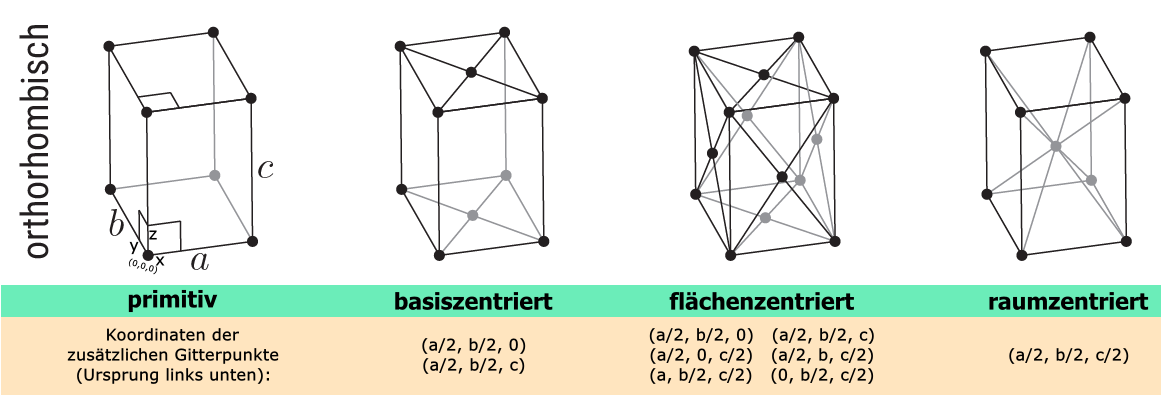
\includegraphics[width=0.7\textwidth]{Ortho.png}
    \caption{\label{fig:orth}}
\end{figure}

\textbf{\textit{b) Wie und warum entstehen bei zentrierten Gittern im Beugungsbild 
systematische Auslöschungen? Wie lauten diese Auslöschungsregeln?}}\\
$\rightarrow$